\documentclass[11pt]{extreport}
\usepackage{geometry}
\usepackage{ragged2e}
\usepackage{titlesec}
\usepackage{indentfirst}
\usepackage{tikz}
\usepackage{array}
\usepackage{amssymb}
\usepackage{amsfonts}
\usepackage{listings}
\usepackage{xcolor}
\usepackage{inconsolata}
\usepackage{ragged2e}
\usepackage{tabularray}
\usepackage{booktabs}
\usepackage{multirow}
\usepackage{amsmath}
\usepackage[backend=biber,style=apa]{biblatex}
\usepackage{float}
\usepackage{hyperref}
\usepackage{graphicx}
\usepackage{caption}
\usepackage{subcaption}
\usepackage[ddmmyyyy]{datetime}

\addbibresource{references.bib}


\geometry{
    a4paper,
    total={6.5in, 10.4in},
}

\titleformat{\chapter}[display]{\Large\bfseries}{\chaptername\ \thechapter}{1em}{\Large}


\begin{document}
	\pagenumbering{gobble}
	\begin{center}
		\huge {
			\textbf{Pruning in Deep Architectures \\
			A detailed study on the methods of pruning in deep architectures }
			
		}
		\vspace{6em}
		\large \textit{Submitted to the University of Kerala in partial fulfillment of the requirements for the completion of Third Semester MSc Computer Science (Artificial Intelligence)}

		\vspace{9em}
		
\includegraphics[scale=1.35]{Logo_of_University_of_Kerala.png}
		\vspace{7em}

		\large{
			BY\\
			\textbf{Hrishikesh M Jayakrishnan}\\
			\textbf{(97424607010)}\\
			\vspace{4em}
			\textbf{Department of Computer Science}\\
			\textbf{University of Kerala}\\
			\textbf{Kariavattom, Thiruvananthapuram, Kerala - 695581}
		}
	\end{center}
	\newpage
	\begin{center}
		\textbf{DEPARTMENT OF COMPUTER SCIENCE}\\
		\textbf{UNIVERSITY OF KERALA}\\
		\textbf{THIRUVANANTHAPURAM, KERALA, 695581}

		\vspace{7em}
		
\includegraphics[scale=1.2]{Logo_of_University_of_Kerala.png}

		\textbf{CERTIFICATE}
		\vspace{4em}

		\justifying
			\noindent This is to certify that the case study and seminar entitled \textbf{Pruning in Deep Architectures: A detailed study on the methods of pruning in deep architectures}, is the bonafide record work done by \textbf{HRISHIKESH M JAYAKRISHNAN (97424607010)} in partial fulfillment of the requirements for the completion of \textbf{Third Semester M.Sc. Computer Science with specialization in Artificial Intelligence}, at the \textbf{Department of Computer Science, University of Kerala, Thiruvananthapuram.}

	\end{center}

	\vspace{6em}

	\noindent
	\begin{minipage}{6cm}
		Internal Guide\\
		\textbf{Dr Aji S}\\
		Associate Professor\\
		Department of Computer Science\\
		University of Kerala\\
	\end{minipage}
	\hfill
	\begin{minipage}{6cm}
		\vspace{1em}
		\begin{flushright}
			\textbf{Dr Aji S}\\
			Head of the Department\\
			Department of Computer Science\\
			University of Kerala\\
		\end{flushright}
	\end{minipage}

	\vspace{3em}
	Date: \today


	\chapter*{
		\begin{center}
			ACKNOWLEDGEMENT
		\end{center}
	}
	\justifying \Large{
		I would like to express my sincere and heartfelt thanks towards all those who have helped me in making this case study. 

		I would like to thank my guide \textbf{Dr Aji S}, who is also the Head of the Department of Computer Science, for his valuable suggestions and vital encouragement. I would also like to extend my gratitude to my course coordinator \textbf{Dr Vidhya M}, for the timely advice and help. 

		I also extend my heartfelt thanks to all \textbf{faculty members} of the department of computer science and to my \textbf{friends}. 
	}

	\newpage

	\chapter*{
		\begin{center}
			DECLARATION
		\end{center}
	}

	\justifying I hereby declare that this case study work titled “Pruning in Deep Architectures - A detailed study on the methods of pruning in deep architectures” is completed by me under the guidance of Dr. Aji S, Associate Professor and Head of the Department, Department of Computer Science, University of Kerala. I hereby declare that the entire report is my own, and not copied from any other work. I am also declaring that this report or any part of it is not submitted for assessment in University of Kerala or any other institution for the same purpose.

	\vspace{5em}

	\noindent
	\begin{minipage}{6cm}
		Place: Karyavattom\\
		Date: \today
	\end{minipage}
	\hfill
	\begin{minipage}{5.76cm}
		\textbf{\large Hrishikesh M Jayakrishnan}
	\end{minipage}



	\newpage

	\chapter*{\begin{center}
		ABSTRACT
	\end{center}}
	\begin{center}
		\justifying{
			Pruning is the process of removing redundant or less important connections from deep neural networks to reduce its size and computational requirements while maintaining its performance. Pruning is considered more surgical than other model compression techniques, such as quantization or distillation. Pruning can be applied in two ways - train-time pruning and post-training pruning, based on when the pruning is done. Train-time pruning involves pruning the model during training process whereas post-training pruning involves pruning the model after it has trained to convergence. This work presents a detailed study of SNOWS(Stochastic Newton Optimal Weight Surgeon), a one-shot post training pruning algorithm which aims at applying layer wise pruning in models taking into account deeper network representations. It uses a hessian free optimization to calculate the newton updates without storing or computing the whole hessian matrix. The SNOWS algorithm can also be applied on top of any sparse mask created from other pruning methods. This study analyzes the working of the SNOWS algorithm.
		}
	\end{center}

	\newpage
	\tableofcontents
	
	\newpage
	\pagenumbering{arabic}
	\setcounter{page}{1}
	\chapter[Introduction]{Introduction}
		Deep learning has revolutionized artificial intelligence, giving computers the ability to extract and learn complex patterns from data through the use of deep neural networks which consists of multiple hidden layers When it comes to understanding images, specific models—like Convolutional Neural Networks (CNNs) (\cite{lecun1998gradient}), ResNets (\cite{he2015resnet}), and the even more powerful Vision Transformers (ViTs) (\cite{dosovitskiy2021vit}), are doing incredibly advanced work. 


		To achieve state-of-the-art performances in various deep learning tasks, people go for building large models with many deep layers, that are capable of capturing very deep features from data. Such models contain more than 25-30 million parameters, and may require high storage and computational needs. Deploying such models in resource-constrained environments like edge devices, mobile platforms, etc is a challenging task.
		
		To address these challenges, different model compression techniques are used. These include quantization - a technique that reduces the precision of numerical values such as weights and activations of a model in order to make them faster (\cite{web_01}), distillation - it is a technique mainly used for transfering a large pre-trained "teacher model" to a smaller "student model" (\cite{web_02}), pruning - it is the process of removing redundant or less important connections from deep neural networks to reduce its size and computational requirements while maintaining its performance. Pruning can be done either after training or before training a model. 

		Some of the existing pruning algorithms use magnitude based pruning or layer wise pruning that preserve local weights only. Some methods may also require training the resulting pruned model to regain their lost accuracy. This report presents a detailed study of the SNOWS algorithm (\cite{lucas2025preserving}). The SNOWS algorithm is a one-shot post-training pruning technique. It applied layer wise pruning while accounting for non-linear activations deep in the network. The algorithm also uses a Hessian-free optimization to compute exact Newton descent steps without needing to compute or store the full Hessian Matrix.

	\newpage
	\chapter[Problem Statement]{Problem Statement}
		Modern deep neural networks contain more number of parameters,resulting in an increased demand for computational resources and increased challenges for deploying in resource constrained devices. To address this, various model pruning methods are used. Fine pruning (\cite{BINGHAM2025101242}) is one such algorithm which uses activation magnitudes to find and remove redundant nuerons. Another algorithm that introduces a training-dynamics aware pruning is WideTopo (\cite{DENG2026108136}) which uses Neural Tangent Kernel(NTK) trace estimation and saliency based scores to preserve structural stability while pruning. In large language models, algorithms like Wanda (\cite{wanda}) uses weight activation based scoring to apply one shot pruning without retraining. Even though these algorithms can effectively prune a neural network, retraining the model is required at some point, for regaining the lost accuracy. Other existing approaches rely on neuron activation statistics, first order gradient information, layer wise pruning that do not consider the effects of a pruned layer on its succeeding layers. 
		
		\vspace{1em}
		Considering the limitations of the existing pruning algorithms, the problem addressed in this case study can be stated as follows:

		\begin{quote}
			\textit{To create an efficient pruning algorithm that reduces the size of deep neural networks while preserving their accuracy and performance on various tasks.}
		\end{quote}


	\newpage
	\chapter[Literature Review]{Literature Review}

	\cite{11092769} has proposed a pruning algorithm that applies structured pruning and weight quantization during training of a neural network. The algorithm GETA (\cite{11092769}) uses three learnable parameters \(q_m, t, \text { and } d\) for calculating the optimal quantization bit-width for each layer. The algorithm then performs structured pruning using a proposed Quantization Aware Dependency Graph to handle complex branches added by quantization operations. The algorithm then employs a 4-stage QASSO or Quantization-Aware Structured Sparse Optimizer for pruning and quantization. The four stages include warm-up, finding feasible bit width using Partial Projected Stochastic Gradient, joint pruning and quantization and finally training the pruned and quantized model till convergence.

	Similarly, \cite{DENG2026108136} has proposed another pruning algorithm that performs pruning during the training of a neural network. WideTopo (\cite{DENG2026108136}) is a foresight pruning technique that finds a small, high-performing sub-network within a larger network before training begins, using a binary mask. WideTopo calculates a combined saliency score for deciding which parameters are important, by giving an input batch of data to the model that has to be pruned. This combined saliency score is a weighted sum of the Neural Tangent Kernel (NTK) (measure of how much a parameter impacts the model's generalization) and the Implicit Target Alignment (ITA) (measure of how much a parameter affects the model's directional inductive bias). By multiplying a decay factor with the saliency score, the algorithm can prevent pruned models from being too narrow by exploring wider topologies during pruning. The model is not pruned once instead it is pruned and regrown for a set number of iterations, followed by a final pruning step to reach the target density.

	Another algorithm inspired by biological neural networks, called as Fine-pruning is proposed by \citeauthor{BINGHAM2025101242}. Fine-pruning is a post training pruning algorithm which personalizes machine learning models for individual users while maintaining overall performance. The algorithm starts with a large pre-trained base model. A small amount of user-specific data called target data is collected. The algorithm then feeds the data one sample at a time using only forward passes, without backpropagation or gradient calculation. The activation maps of each layer are recorded, and the contribution of each individual weight is calculated by summing its activation values across all input samples. Weights that contribute the least to the output are pruned by setting them to zero.

	\newpage
	\chapter[Methodology]{Methodology}

		The SNOWS\footnote{Stochastic Newton Weight Optimal Surgeon} algorithm is a one-shot, post-training pruning framework that accurately adjusts the values of a network's remaining weights (after a sparse mask is already applied) to recover performance without requiring expensive retraining. It accomplishes this by optimizing a new, more global reconstruction objective, while also considering the non-linear activations and other connections present deep within neural networks. This complex non-linear problem is then solved using a specialized Hessian-Free second order optimization method.

		Consider a neural network with \(L\) layers. The function of this neural network can be represented as \(f(X^0, W)\), where 
		
		\noindent \(W = (W^1, W^2, W^3, \ldots, W^L)\) is the collection of weight matrices upto \(L\) layers and \(X^0\) is the input data. For a layer \(\ell\), the output can be calculated as \(Y^{\ell} = f^{\ell}(X^{\ell},W^{\ell})\). If we consider a loss function that is twice differentiable, given the weight parameters \(W\), the gradient can be denoted as 
		
		$$\nabla \mathcal{L}(W) = \frac{\partial \mathcal{L}}{\partial W} $$
		
		and the hessian can be denoted as 

		$$H = \frac{\partial^2 \mathcal{L}}{\partial W^2}$$



		The authors have formulated a layer wise objective function that considers the non-linear activations and other connections that follow the layer being pruned.

		\begin{equation} \label{eq1}
			\min_{\widehat{W}^l \in \mathcal{W}} \mathcal{L}(\widehat{W}^l) := \sum_{k=0}^{K} \left\lvert\left\lvert Y^{l+k} - f^{l:l+k}(X^l, \widehat{W}^l)\right\rvert\right\rvert_2^2
		\end{equation}


		Here, \(f^{\ell:\ell + k}(\cdot) \) can be defined as a composition of the next k operations starting from layer \(\ell\):

		$$f^{\ell:\ell + k}(X^{\ell},W^{\ell}) = f^{\ell + k}(\cdot, W^{\ell + k}) \circ f^{\ell + k - 1}(\cdot, W^{\ell + k - 1}) \circ \ldots \circ f^{\ell}(\cdot, W^{\ell}) $$ 

		The gradient of the loss function with respect to the pruned weights \(\widehat{W}^l\) can be expressed as:

		\begin{equation} \label{eq2}
			\nabla \mathcal{L}(\widehat{W}^l) = \sum_{k=0}^{K} \left[ -2(Y^(l+k) - f^{l:l+k}(X^l, \widehat{W}^l))\frac{\partial f^{l:l+k}(X^l,\widehat{W}^l)}{\partial \widehat{W}^l} \right]
		\end{equation}


		An advantage of this equation is that it decreases memory requirements for computing the full network requirements. Since we consider only the operations starting from layer \(\ell\) to \(\ell + k\) instead of the whole network, the number of activations that are to be constructed is minimized, resulting in a shortened computational graph required for calculating the gradient. Even if we use a layer wise function, computing all the second order partial derivatives of \(f^{\ell: \ell+k}\) for \(k = 0, 1, \ldots, K\) to form the Hessian is not possible for larger networks.

		The authors have proposed a second order optimization framework to optimize the layer wise objective function in \ref{eq1}. The algorithm initially assumes a sparse mask is already applied, using existing methods like magnitude pruning, optimal brain compression, etc. 

		The problem is then decoupled into a bi-level optimization problem,

		\begin{equation} \label{eq3}
			\min_{Z \in \mathcal{Z}} \min_{\widehat{W}_Z^l \in \mathbb{R}^{d_{l-1} \times d_l}} \mathcal{L}(\widehat{W}_Z^l) = \sum_{k=0}^{K} ||Y^{l+k} - f^{l:l+k}(X^l, \widehat{W}_Z^l \odot Z)||_2^2
		\end{equation}


		To solve the continuous problem, the method uses a second-order Taylor expansion of the new objective function around the current weights $\widehat{W}_Z^l$.
		
		\begin{equation} \label{eq4}
			\mathcal{L}(\widehat{W}_Z^l + \delta_Z) \approx \mathcal{L}(\widehat{W}_Z^l) + \nabla\mathcal{L}(\widehat{W}_Z^l)^T \delta_Z + \frac{1}{2}\delta_Z^T H_Z \delta_Z
		\end{equation}

		Minimizing the taylor expansion with respect to $\delta_Z$ gives

		\begin{equation} \label{eq5}
			min_{\delta Z} \left\{{\delta^{T}_Z} \nabla L(\widehat{W}^{l}_Z) + \frac{1}{2} \delta^{T}_Z H_Z \delta_Z \right\}
		\end{equation}

		Setting the above gradient to zero gives us

		\begin{equation} \label{eq6}
			\nabla \mathcal{L}(\widehat{W}^{l}_Z) + H_Z \cdot \delta_Z = 0
		\end{equation}

		\begin{equation}\label{eq7}
			H_Z \cdot \delta_Z = -\nabla\mathcal{L}(\widehat{W}_Z^l)
		\end{equation}

		From equation \ref{eq7} obtained we can calculate the Newton update $\delta_Z$ as follows:

		$$\delta_Z = -H_Z^{-1} \nabla\mathcal{L}(\widehat{W}_Z^l)$$

		Calculating the inverse of the Hessian matrix $H_Z$ is computationally expensive and infeasible for large neural networks. To address this, SNOWS uses a Hessian-Free method to solve the equation without explicitly computing or storing the Hessian matrix. The authors use the conjugate gradient method (\cite{ref1})

		We add a small dampening term $\lambda I$ to the Hessian matrix to ensure it is positive definite.
		$$(H_Z + \lambda I) \delta_Z = -\nabla\mathcal{L}(\widehat{W}_Z^l)$$

		Consider the equation above as a linear system of equations $A x = b$, where $A = H_Z + \lambda I$, $x = \delta_Z$, and $b = -\nabla\mathcal{L}(\widehat{W}_Z^l)$. We initialize $\delta_Z$ to zero and compute the initial residual $r_0 = b - A \delta_Z$ and the initial search direction $p_0 = r_0$. Then, for each iteration $k$, we perform the following steps:
		\begin{enumerate}
			\item Compute \(\alpha_0 = \frac{r^{T}_0 \cdot r_0}{p^{T}_0 \cdot Ap_0}\)
			\item Update \(\delta_Z = \delta_Z + \alpha_0 p_0\)
			\item Update residual \(r_1 = r_0 - \alpha_0 Ap_0\)
			\item Repeat the above steps for a fixed number of iterations.
		\end{enumerate}

		Finally, the calculated update $\delta_Z$ is then used to adjust the remaining weights after pruning, which helps in recovering the performance of the pruned model without requiring retraining. 

		The algorithm performs two types of pruning - unstructured pruning and semi-structured pruning. Unstructured pruning involves pruning individual weights in an unrestricted format, resulting in high compression of model. While semi-structured pruning use \(N:M\) sparsity, where every \(N\) neurons out of every \(M\) contiguous neurons are retained. The SNOWS algorithm is applied on two pre-trained CNN (\cite{lecun1998gradient}) models. The first one is ResNet-20 pre-trained on the CIFAR-10 (\cite{cifar}) dataset, while the second one is ResNet-50 where three versions, pre-trained on the CIFAR-10, CIFAR-100 (\cite{cifar}) and ImageNet-1K (\cite{data_01}), are used
		

	\newpage
	\chapter[Experiment Analysis]{Experiment Analysis}

		\subsection[Experiment Setup]{Experiment Setup}
		The pruning is applied on the ResNet models using a single 16gb Nvidia RTX 5060ti GPU. 

		\subsection[Dataset]{Dataset}

		Below are the datasets used for the purpose of pruning the models.
		
		\begin{enumerate}
			\item CIFAR-10 (\cite{cifar}) - The CIFAR-10 dataset consists of 60000 32x32 colour images in 10 classes, with 6000 images per class. The dataset is split into 50000 training images and 10000 test images.
			\item CIFAR-100 ({\cite{cifar}}) - The CIFAR-100 dataset is similar to the CIFAR-10 dataset but contains 100 classes with 600 images each. This dataset is also split into 50000 training images and 10000 test images.
			\item Mini-ImageNet 1K (\cite{data_01}) - This dataset is a mini version of the original ImageNet 1K dataset. It consists of 1000 classes of images with \(\sim37\) images in each class
		\end{enumerate}

		\subsection[Evaluation Metrics]{Evaluation Metrics}
		Below are the evaluation metrics used for the study
		\begin{enumerate}
			\item Accuracy - The accuracy is measured by calculating the ratio of correct predictions to the total predictions made by the deep learning model.
			\item Total Pruning Time - It is obtained by measuring the total wall-clock time required for pruning a deep learning model.
		\end{enumerate}
		\newpage
		\subsection[Quantitative Analysis]{Quantitative Analysis}
			The tables below shows the accuracies of the two models pre-trained on the CIFAR-10 (\cite{cifar}), CIFAR-100 (\cite{cifar}) and Mini-ImageNet 1K (\cite{data_01}). The results compare the accuracies of the base dense model with their pruned version, according to the various values of $K$ and sparsity levels. The results also include the pruning time taken for each model in unstructured pruning and semi-structured or \(N:M\) pruning.
			\begin{table}[H]
				\centering
				\caption{Accuracy of models on N:M Pruning}
				\begin{tabular}{lcccccc} 
					\toprule
					\multirow{3}{*}{K} & \multicolumn{2}{c}{ResNet-20} & \multicolumn{2}{c}{Resnet50} & \multicolumn{2}{c}{Resnet50}   \\
									& \multicolumn{2}{c}{CIFAR-10} & \multicolumn{2}{c}{CIFAR-10} & \multicolumn{2}{c}{CIFAR-100}  \\ 
					\cmidrule{2-7}
									& 1:4     & 2:4                & 1:4    & 2:4                 & 1:4     & 2:4                  \\ 
					\hline
					Base Accuracy      & \multicolumn{2}{c}{92.59\%}  & \multicolumn{2}{c}{94.64\%}  & \multicolumn{2}{c}{77.42\%}    \\ 
					\midrule
					k = 10             & 79.98\% & 90.6\%                    & 94.33\%& 94.5\%                       & 72.83\% & 77.14\%\\
					k = 20             & 81.39\% & 90.56\%                   & 94.32\%& \textbf{94.53\%}             & 74.31\% & 77.07\%\\
					k = 40             & \textbf{84.55\%} & \textbf{91.7\%}  & \textbf{94.4\%} & 94.49\%             & \textbf{74.61\%} & \textbf{77.2\%}               \\
					\bottomrule 
				\end{tabular}
				\label{table1}
			\end{table}

			Table \ref{table1} shows the results of \(N:M\) pruning on ResNet models. As the value of \(K\) increaseas, more number of activations are considered ahead of a layer that is being pruned, resulting in higher accuracy of the ResNet models.

			\begin{table}[H]
				\centering
				\caption{Accuracy of models on Unstructured Pruning}
				\begin{tabular}{lccc} 
					\toprule
					K = 40   & ResNet-20 on CIFAR-10 & ResNet-50 on CIFAR-10 & \multicolumn{1}{l}{ResNet-50 on CIFAR-100}        \\ 
					\midrule
					Sparsity & Base Accuracy = 92.59\% & Base Accuracy = 94.64\% & \multicolumn{1}{l}{Base Accuracy = 77.41\%} \\
					\midrule
					0.5      & \textbf{92.63\%} & 94.36\% & \textbf{76.55\%}             \\
					0.6      & 91.54\% & \textbf{94.5\%} & 76.19\%               \\
					0.7      & 88.65\% & 94.46\% & 75.03\%                         \\
					\bottomrule
				\end{tabular}
				\label{table2}
			\end{table}

			\begin{table}[H]
				\centering
				\caption{Accuracy of model Unstructured Pruning}
				\begin{tabular}{lc} 
					\toprule
							& \begin{tabular}[c]{@{}c@{}}ResNet-50 on ImageNet\\(K=2)\end{tabular}  \\ 
					\midrule
					Sparsity & Base Accuracy = 75.68\%      \\          
					\midrule                              
					0.5      & \textbf{73.28\%}                                                              \\
					0.6      & 67.55\%                                                              \\
					0.7      & 58.22\%                                                              \\
					\bottomrule
				\end{tabular}
				\label{table3}
			\end{table}

			Tables \ref{table2} and \ref{table3} showcase the accuracy obtained on ResNet-20 and ResNet-50, by applying unstructured pruning. Here, for increasing model sparsity, the resulting accuracy decreases because of the increase in amount of neurons that have zero weights.

			\begin{table}[H]
				\centering
				\caption{Total Pruning Time in minutes (1:4 Pruning)}
				\begin{tabular}{lccc} 
					\toprule
					& ResNet-20 on CIFAR-10 & ResNet-50 on CIFAR-10 & \multicolumn{1}{l}{ResNet-50 on CIFAR-100}  \\ 
					\cmidrule{2-4}
					K  & Time                 & Time                 & Time                                       \\ 
					\midrule
					10 & 6.3            & 14.1           & 17.9                                 \\
					20 & 11.5           & 16.3           & 28.3                                 \\
					40 & 24.2           & 16.9           & 35                                   \\
					\bottomrule
				\end{tabular}
				\label{table4}
			\end{table}



			\begin{table}[H]
				\centering
				\caption{Total Pruning Time in minutes (2:4 Pruning)}
				\begin{tabular}{lccc} 
					\toprule
					& ResNet-20 on CIFAR-10 & ResNet-50 on CIFAR-10 & \multicolumn{1}{l}{ResNet-50 on CIFAR-100}  \\ 
					\cmidrule{2-4}
					K  & Time                 & Time                 & Time                                       \\ 
					\midrule
					10 & 6.8            & 12.9           & 20.8                                 \\
					20 & 14.5           & 15.6            & 37.3                                    \\
					40 & 13.4           & 18.7           & 44.9                                \\
					\bottomrule
				\end{tabular}
				\label{table5}
			\end{table}

			\begin{table}[H]
				\centering
				\caption{Total Pruning Time in minutes (Unstructured Pruning with \(K = 40\))}
				\begin{tabular}{lccc} 
					\toprule
					& ResNet-20 on CIFAR-10 & ResNet-50 on CIFAR-10 & \multicolumn{1}{l}{ResNet-50 on CIFAR-100}  \\ 
					\cmidrule{2-4}
					Sparsity  & Time                 & Time                 & Time                                       \\ 
					\midrule
					0.5 & 6              & 15.3              & 33                                    \\
					0.6 & 7              & 10.8               & 22.2                                    \\

					0.7 & 8              & 8.8              & 16.6                                    \\
					\bottomrule
				\end{tabular}
				\label{table6}
			\end{table}

			Tables \ref{table4} and \ref{table5} represents the total time taken for applying \(N:M\) pruning on the CNN models. For increasing number of \(K\), the total pruning time of a model increases, as we need to consider more number of activations ahead. 

			In unstructured pruning, at a fixed \(K\) value, table \ref{table6}
			shows a decrease in pruning time for higher sparsity levels. This is due to higher number of weights being zero.



		
		\newpage
		\subsection[Qualitative Analysis]{Qualitative Analysis}
			Each figure compares the classification done by a pre-trained ResNet model and best models obtained through \(N:M\) pruning and unstructured pruning.
			\begin{figure}[H]
				\begin{center}
					\begin{subfigure}[b]{0.4\textwidth}
						\captionsetup{justification=centering}
						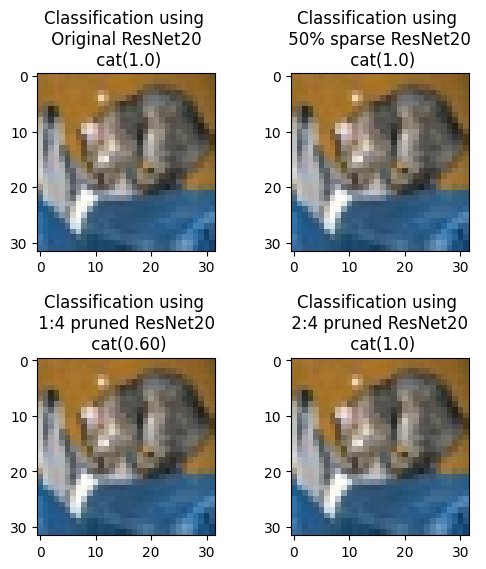
\includegraphics[scale=0.6]{output1.png}
						\caption{Comparison of accuracies of original ResNet-20 with pruned versions of ResNet-20, using CIFAR-10}
					\end{subfigure}
					\hfill
					\begin{subfigure}[b]{0.4\textwidth}
						\captionsetup{justification=centering}
						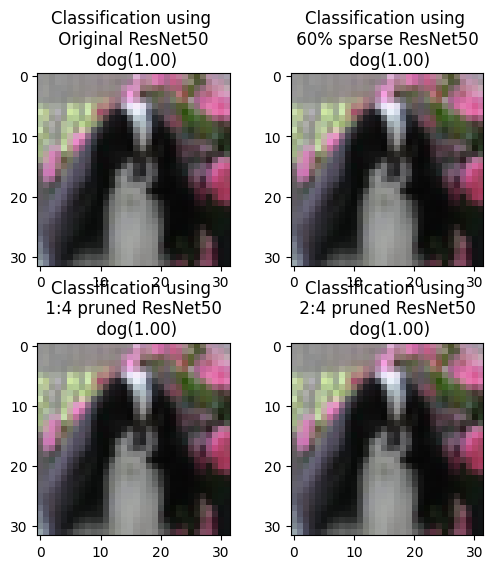
\includegraphics[scale=0.6]{output2.png}
						\caption{Comparison of accuracies of original ResNet-50 with pruned versions of ResNet-50, using CIFAR-10}
					\end{subfigure}
				\end{center}
			\end{figure}

			\begin{figure}[H]
				\begin{center}
					\captionsetup{justification=centering}
					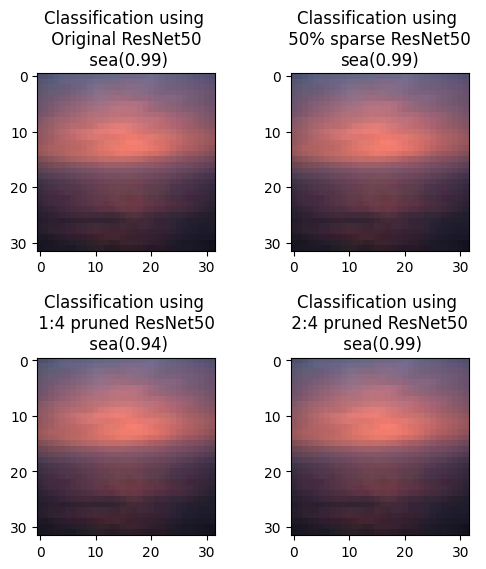
\includegraphics[scale=0.6]{output3.png}
					\caption{Comparison of accuracies of original ResNet-50 with pruned versions of ResNet-50, using CIFAR-100}
				\end{center}
			\end{figure}

			The above results show that the pruned models are also able to correctly classify the input image, performing on par with the pre-trained model.
	\newpage
	\chapter[Conclusion]{Conclusion}
		In this study, we conduct a thorough analysis on some of the modern pruning algorithms applied in deep architectures. Pruning is a crucial technique for optimizing deep neural networks, enabling reduced model size, faster inference, and improved generalization. Various pruning algorithms, such as WideTopo, GETA, and Fine-Pruning, offer different approaches to achieve these goals, each with its own strengths and limitations. The SNOWS algorithm presents a novel approach to pruning by utilizing a Hessian-Free second-order optimization method to adjust remaining weights after pruning, effectively recovering performance without retraining.

	\newpage
	\printbibliography
\end{document}